\chapter{\label{chap:modelagem}Modelagem}
A diretriz do desenvolvimento deste trabalho seguirá algumas propostas da metodologia Kanban. Desenvolvido no final da década de 1940 pela Toyota, o método Kanban apresenta ferramentas que diminuem o trabalho em progresso (\textit{work in process}) e  auxiliam na administração de custos e na identificação de gargalos e outros impedimentos no fluxo do desenvolvimento do processo \cite{GROSS2003}. Um processo guiado por Kanban terá suas características, peculiaridades e riscos destacados, possibilitando ao time uma rápida percepção dos possíveis problemas e oportunidades que determinada atividade poderá apresentar.

Essa é "uma técnica que traduz em linhas, colunas e cartões coloridos o fluxo existente no processo de produção"\ \cite{AUDY2015}. Palavra do idioma japonês, \textit{kanban} significa "quadro"\ \cite{GROSS2003} e este é o seu componente essencial -- um quadro com diversas colunas onde cada uma delas representa o estado de algum processo do projeto, como ilustrado na Figura ~\ref{fig:kanban1}. Por ser uma ferramenta sucinta e visual, uma rápida visualização do painel de tarefas deve permitir que se obtenha conhecimento de aspectos como: informações básicas sobre o processo; o estágio de cada um deles e qual sua prioridade ou nível de dificuldade, os quais são usualmente indicados por cores diferentes \cite{AUDY2015}. 

Todos estes aspectos devem ser previamente definidos pelo time durante o processo de projeção do \textit{kanban}. Cada projeto possuirá um \textit{kanban} específico de acordo com seu escopo e sua equipe, sendo delegadas funções para cada integrante do time. Outro fator que deve ser definido são os limitadores, os quais definirão algumas regras para o fluxo do desenvolvimento do processo, como o número máximo de tarefas na fila de testes, entre outros \cite{AUDY2015}. Assim, cada integrante do time é responsável por manter o ritmo do processo e evitar que tarefas acumulem.

\begin{figure}[htb]
\centering
\caption[\emph{Kanban}]{\label{fig:kanban1}\emph{Kanban} criado na ferramenta Trello}
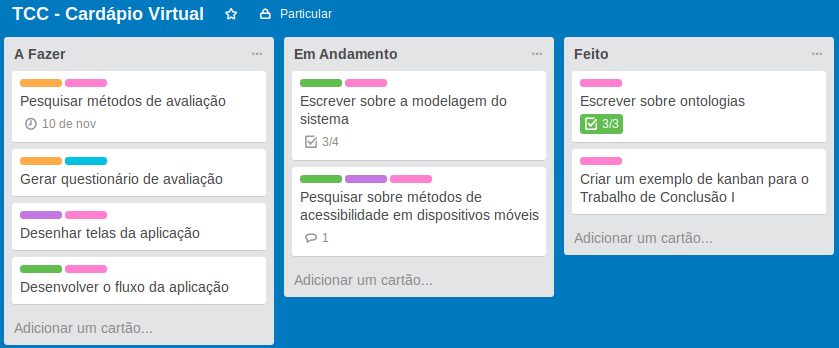
\includegraphics[width=0.8\textwidth]{fig/kanban1.png}
\end{figure}


\section{Planejamento}
Ao realizar o planejamento de um software, podem surgir alguns conflitos entre as diferentes partes interessadas. É possível que o cliente, o usuário, o desenvolvedor e outros integrantes do projeto tenham visões diferentes sobre o mesmo projeto e o resultado não venha a ser satisfatório para um dos lados \cite{COHN2004}. Neste caso, busca-se por uma forma em que todas as partes possam trabalhar juntas e entrar em um consenso e, para isso, é necessário que a equipe não aja de forma autocentrada e leve em consideração quem é seu usuário, o que ele quer e como ele se comporta \cite{AUDY2015}. Por isso, duas técnicas foram escolhidas para auxiliar no planejamento deste trabalho: o desenvolvimento de \textit{personas} e o uso de \textit{histórias de usuário}.


\section{Personas}

Conhecer e criar empatia com quem usufruirá do sistema são atividades necessárias, apesar de ainda pouco praticadas em algumas áreas do desenvolvimento de software. Uma forma de registrar informações acerca do cliente é a partir da criação de personas -- perfis fictícios de possíveis usuários do sistema a ser desenvolvido. Cada persona possui um nome, um perfil, um comportamento e um conjunto de necessidades que deseja suprir; sendo importante entender e traçar diferentes tipos de clientes, como um usuário comum e um usuário administrador, por exemplo \cite{AUDY2015}. Desta forma, esses perfis representarão uma parcela significativa dos clientes em potencial.

\cite{ERGO2015} destacam que
\begin{directcite}
    quando se pensa em análise para acessibilidade, o objetivo é conhecer os perfis dos futuros usuários de um sistema que são portadores de deficiência. (...) Assim, uma boa ideia é a elaboração de "personas"\ descrevendo o perfil de usuários portadores de deficiência e de "cenários problema"\ descrevendo as estratégias e o ambiente de trabalho atuais. 
    Essas personas e esses cenários seriam usados nas atividades de especificação e concepção da interface.
\end{directcite}
Tendo em vista a importância desta prática, as seções seguintes apresentarão três perfis de possíveis usuários do sistema a ser desenvolvido.

\subsection{Pessoa com Deficiência Visual em Busca de Restaurantes nas Proximidades}
Airy Gavião é estudante do curso de Sistemas de Informação em sua universidade. Com 22 anos, ela está no fim de sua graduação, mas, durante todos esses anos, Airy não possuía o costume de frequentar os bares e restaurantes das redondezas do prédio onde estudava, uma vez que não os considerava acessíveis para pessoas com deficiência visual. Normalmente, Airy trazia algum lanche que preparara em casa; evitava ter que comer em algum estabelecimento, uma vez que considerava ser um incômodo o ato de perguntar aos seus amigos quais eram as características das comidas apresentadas nos balcões das lancherias. 

Ao baixar o aplicativo de auxílio em restaurantes, Airy procurou pelos restaurantes e bares em sua proximidade, buscando por algum que possuísse registro no sistema. Os nomes dos restaurantes registrados foram listados ao usuário, o qual selecionou o primeiro da lista para conferir as informações básicas do local e seu cardápio. Por não comer carne, Airy deu preferência pelo acesso dos itens vegetarianos, apenas. Ao perceber que havia algumas opções que lhe agradavam, ela decidiu ir ao restaurante em questão.

Após sua refeição, levando em consideração a proximidade do local e o custo benefício, Airy decidiu adicionar o restaurante em sua lista de "locais favoritos". Para isso, Airy simplesmente acessou a tela de informações adicionais do restaurante e selecionou a opção de \emph{favoritar}.

\subsection{Pessoa com Deficiência Visual em Viagem}
Olinda Muniz é professora em uma pequena comunidade indígena no interior do estado e, apesar de possuir um celular, faz uso de apenas algumas aplicações. Com frequência, ela precisa viajar para outras regiões em congressos ou eventos educacionais e acaba pernoitando nessas cidades. Ao agendar uma viagem para Porto Alegre, a professora decide verificar os cardápios dos restaurantes próximos à Pontifícia Universidade Católica do Rio Grande do Sul, local onde será realizado o evento. Ao inserir o endereço da universidade, os  restaurantes são listados e ela pode acessar seus cardápios. Desta forma, Olinda pode sugerir o restaurante para seus amigos, uma vez que tem conhecimento do que é servido no local. 

\subsection{Alguém que Convive com Pessoas com Deficiências Visuais}
Vãngri Kaingáng, radialista de 30 anos, está em um relacionamento com uma pessoa com deficiência visual. Normalmente, quando decidem sair para jantar, Vãngri acaba lendo o cardápio físico para Rosane, mas percebe que ela não se sente muito a vontade e não faz muitas perguntas; ao encontrar uma opção que pareça agradável, Rosane a escolhe, sem checar outras opções.

Devido a este impasse, Vãngri pedia a seus ouvintes recomendações de restaurantes que fossem mais acessíveis ou sugestões de refeições de acordo com o gosto de Rosane. A partir disso, chegou ao conhecimento da aplicação móvel com cardápio acessível. Rosane acessou a aplicação e buscou pelo nome de restaurantes já conhecidos, analisando seus cardápios e marcando-os como favoritos. Com estas informações contidas na aplicação, Vãngri pode analisar as preferências de Rosane e, através do sistema de busca, encontrar novos restaurantes, cafés, bistrôs, entre outros.

\section{Histórias de Usuário}

Segundo \cite{COHN2004}, uma história de usuário (US -- \emph{User Story}) descreve uma funcionalidade que será valiosa para o usuário do software. Normalmente, segue a seguinte estrutura: \textit{"como um X, eu quero Y, porque Z"}; onde X é a pessoa beneficiada, Y é alguma funcionalidade do sistema e Z é o valor desta funcionalidade. Seguindo este modelo, cada história especifica quem é o usuário, qual sua necessidade e qual sua motivação \cite{AUDY2015}, podendo conter detalhes adicionais. Uma vez que as US são representações de funcionalidades que serão validadas pelo usuário, requisitos não-funcionais, como, por exemplo, a linguagem na qual o programa será desenvolvido, não são incorporados nelas \cite{COHN2004}. As histórias de usuário formuladas para este sistema serão apresentadas a seguir.

\subsection{US01 -- Acessar o sistema}

\textit{"Eu, como um usuário, desejo poder acessar o sistema quando achar necessário."}

Esta história de usuário apresenta a seguinte funcionalidade: a de aceso ao sistema. Com ela, o usuário é livre para entrar no sistema e ter acesso ao seu conteúdo, bem como sair dele. Para realizar tais tarefas, basta selecionar a aplicação e, ao carregá-la em seu dispositivo, informar seus dados de localização, os quais são obtidos através da conexão com o GPS.

\subsection{US02 -- Buscar Restaurante}

\textit{"Como usuário, desejo buscar restaurantes e acessar suas informações,  verificando quais restaurantes estão em minha proximidade e quais alimentos oferecem."}

A habilidade de buscar um restaurante no sistema e poder acessar suas informações é o que compõe esta história de usuário. O cliente deve ser capaz de buscar um restaurante no campo de busca através da inserção de texto ou por um comando de voz e, caso o restaurante esteja registrado no sistema, poderá selecioná-lo, sendo redirecionado à tela que contém as informações gerais do local. 

\subsection{US03 -- Acessar Cardápio}

\textit{"Como usuário, desejo acessar o cardápio dos restaurantes com o intuito de verificar as opções disponíveis e analisar as informações de cada alimento."}

O usuário deverá poder acessar os cardápios dos restaurantes registrados no sistema, bem como informações detalhadas das refeições. Estarão disponíveis os ingredientes de cada item do menu, além de informações adicionais que possam ser relevantes para os clientes.

\subsection{US04 -- Filtrar Cardápio}

\textit{"Eu, como usuário, busco poder filtrar as opções do cardápio de acordo com uma dieta específica, bem como outras categorias."}

O que caracteriza esta história de usuário é a possibilidade de filtrar cardápios de acordo com categorias pré-estabelecidas pelo sistema. Caso o usuário seja vegetariano, por exemplo, ele poderá selecionar a opção que apresenta apenas aqueles produtos que não contêm carne. Assim, a navegação no sistema será mais rápida e objetiva.

\subsection{US05 -- Favoritar Restaurante}

\textit{"Como um usuário, eu desejo poder favoritar certos locais, podendo ter fácil acesso a eles na aplicação."}

Nesta história, representamos a possibilidade de cada usuário ter uma lista pessoal de fácil acesso a locais de sua preferência. Podendo marcar um determinado local como "favorito", este estabelecimento ficará registrado em uma lista à parte, onde o usuário poderá acessá-la na página inicial do sistema. Sendo assim, caso deseje obter informações sobre o local, não será necessário procurar o restaurante no sistema de buscas.

\section{Fluxograma}
Um fluxograma é a representação visual da sequência de passos em um processo, onde diferentes passos são representados por caixas e o encadeamento destes passos é representado por setas \cite{REYNARD1995}. Estes diagramas ajudam a sistematizar um entendimento comum sobre o processo; a visualizar o processo como processos menores, os quais interagem entre si; a melhorar o processo, eliminando ineficiências; e a padronizar este processo, tornando-o mais consistente. Quando se deseja obter um esboço dos passos mais genéricos do processo em questão, \cite{REYNARD1995} indica o uso de um fluxograma básico sem atividades muito detalhadas. Um diagrama contendo estas características é apresentado a seguir, na Figura \ref{fig:fluxograma}.

\begin{figure}[H]
    \centering
    \caption[Fluxograma Geral do Sistema]{\label{fig:fluxograma}Fluxograma geral da aplicação. As setas tracejadas indicam a saída do sistema}
    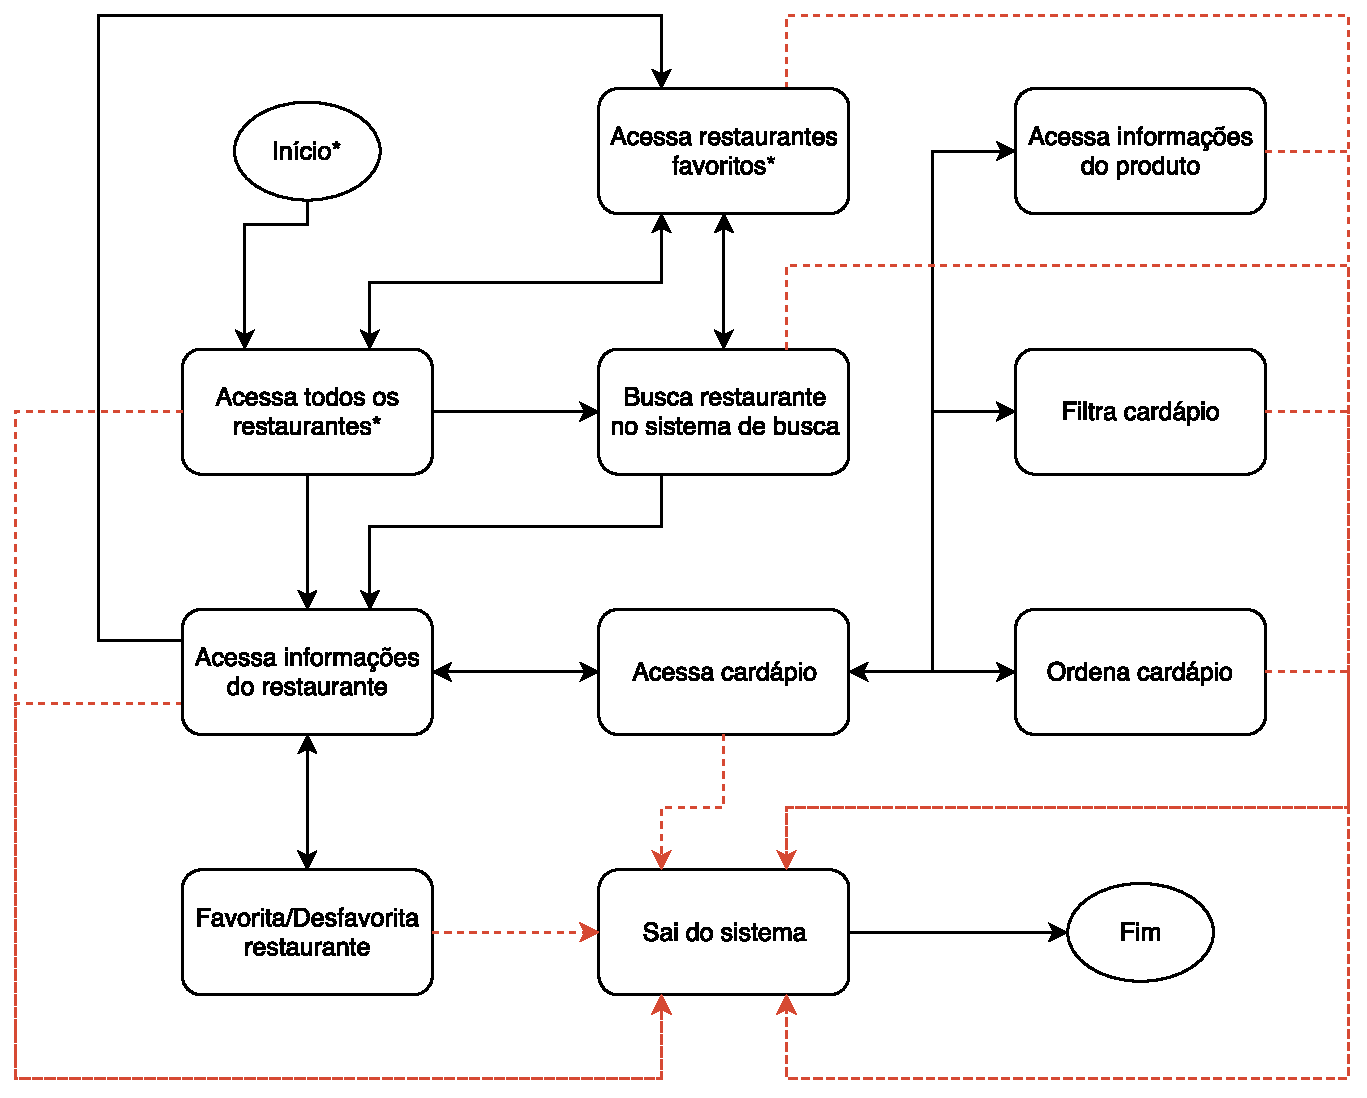
\includegraphics[width=0.9\textwidth]{./pdf/fluxograma-atual.pdf}
\end{figure}


\section{Modelagem do Banco de Dados}

A aplicação desenvolvida neste trabalho não requer uma estrutura de dados muito robusta. O banco de dados aqui desenvolvido é composto por quatro tabelas: \emph{Restaurantes, Logs, Categorias\_Produtos} e \emph{Duvidas}. A tabela de Restaurantes é composta pelos dados básicos de cada localização, bem como suas coordenadas; além disso, também há uma coluna (\emph{Favorito}) que demarca se este restaurante fora marcado como favorito ou não pelo usuário. A tabela de Logs guarda o nome dos produtos e quantas vezes eles foram acessados -- este item será importante para um dos critérios de ordenação do cardápio. Já a tabela Categorias\_Produtos armazena a relação entre os produtos e a categoria a qual eles pertencem, auxliando na construção do cardápio. Por fim, a tabela de Dúvidas é uma estrutura criada para armazenar os dados referentes ao sistema de Ajuda da aplicação. As tabelas descritas previamente e suas relações podem ser vistas na Figura \ref{fig:bd}:

\begin{figure}[H]
	\centering
	\caption[Modelagem do Banco de Dados]{\label{fig:bd}Modelo do banco de dados para o sistema de Cardápios Virtuais}
	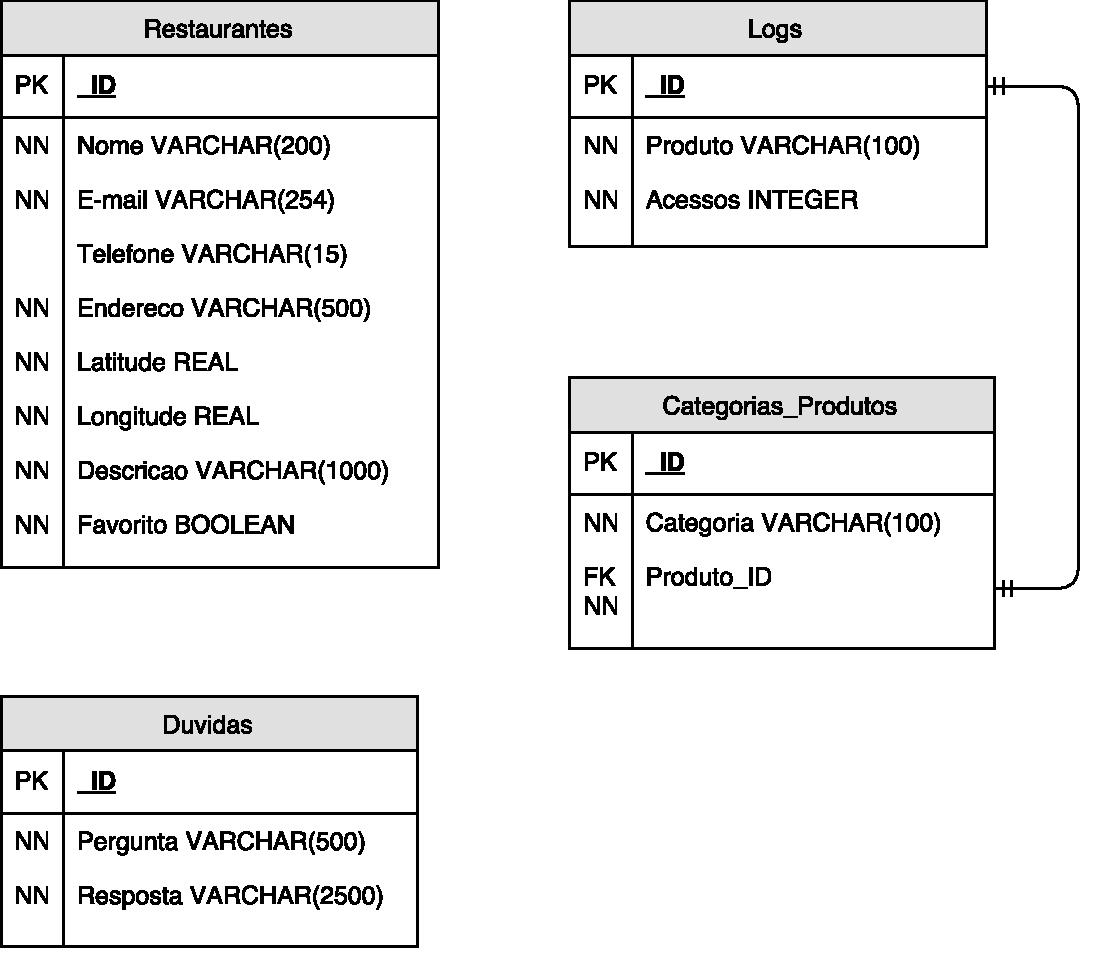
\includegraphics[width=0.9\textwidth]{./pdf/bd.pdf}
\end{figure}

\section{Estrutura de Classes}



\begin{figure}[H]
	\centering
	\caption[Estrutura de Classes]{\label{fig:diagrama-classes}Estrutura de classes geral da aplicação}
	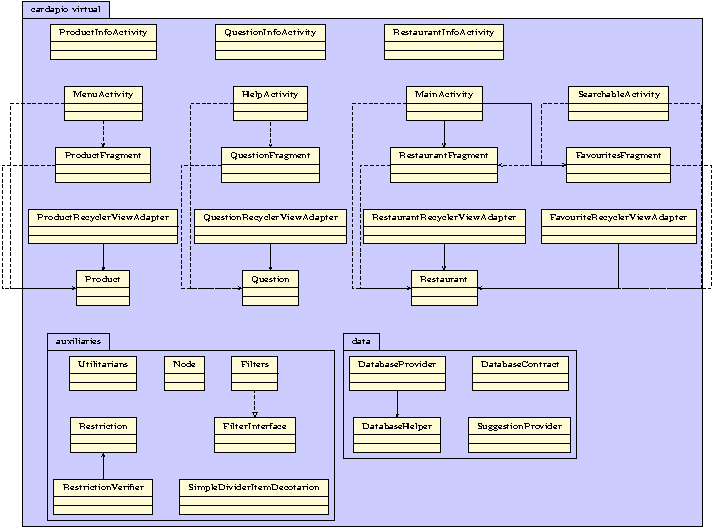
\includegraphics[width=0.9\textwidth]{./pdf/tikz/diagrama-classes.pdf}
\end{figure}
